\documentclass{article}
\usepackage[utf8]{inputenc}

\title{Tarea 3 - Redes de Computadores}
\author{Juan Carlos Arriagada 2973565-4\\Celeste Bertin 201092008-9}
\date{20 de Junio del 2014}

\usepackage{natbib}
\usepackage{graphicx}

\begin{document}

\maketitle

\section{Introducción}
El presente informe tiene por objetivo mostar al lector cual es el camino que sigue la informacion para llegar a su destino, explicando brevemente porque son asi las rutas. Ademas, se espera familiarizar al lector con el algoritmo de Vector-Distancia para el establecimiento de las rutas??? y explicar como es que este algoritmo permite darle robustes a las redes en caso de falla de algun enlace fisico.
\iffalse
I don't want this to happen
\begin{figure}[h!]
\centering
\includegraphics[scale=1.7]{universe.jpg}
\caption{The Universe}
\label{fig:univerise}
\end{figure}

\fi
\section{Desarrollo}
El presente informe se divide en 3 items, los cuales son "vdvds", "bllblabla2" y "blablabla3", los cuales se detallan a continuacion:

\subsection{Parte 1: Open Visual Traceroute }
Los paquetes viajan de un continente a otro a traves de cables submarinos de fibra optica, los cuales transmiten las señales digitales utilizadas para telecomunicaciones internacionales, entre los cuales esta el internet. Estos cables estan instalados entre continentes de tal forma que si se daña alguno, existe redundancia de las conexiones tal que no se pierda comunicacion de caso de contratiempos. 
Chile esta conectado al resto del mundo a traves de varios cables submarinos de fibra optica\citep{website:telegeography}, los cuales son:
\begin{itemize}
  \item Panamericano (PAN-AM)
  \item South America-1 (SAm-1)
  \item South American Crossing (SAC)/Latin American Nautilus (LAN) \ldots
\end{itemize}

Los cuales se pueden ver en la siguiente figura:
\clearpage

\begin{figure}[h!]
\centering
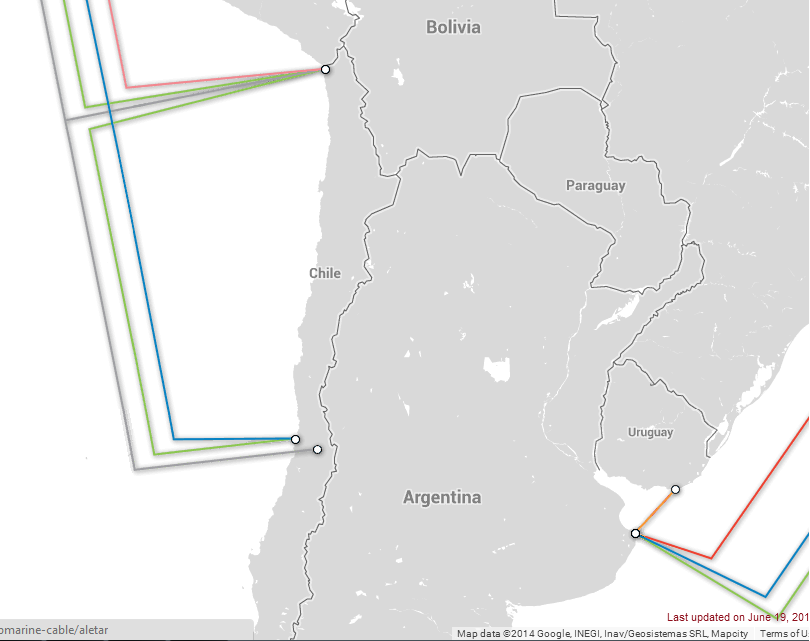
\includegraphics[scale=0.4]{fiber_chile.png}
\caption{Cables submarinos que conectan a Chile a otros continentes}
\label{fig:cables submarinos}
\end{figure}

A continuación se utiliza Open Visual Trace Route 5.1.1 para investigar la ruta tomada por los paquetes al acceder a los siguientes sitios web desde Santiago de Chile:

\begin{description}

  \item[Moodle] \hfill \\
Se ingresó http://moodle.inf.utfsm.cl/ a Open Visual Trace Route, el cual mostró las rutas tomadas para llevar al server final

\begin{figure}[h!]
\centering
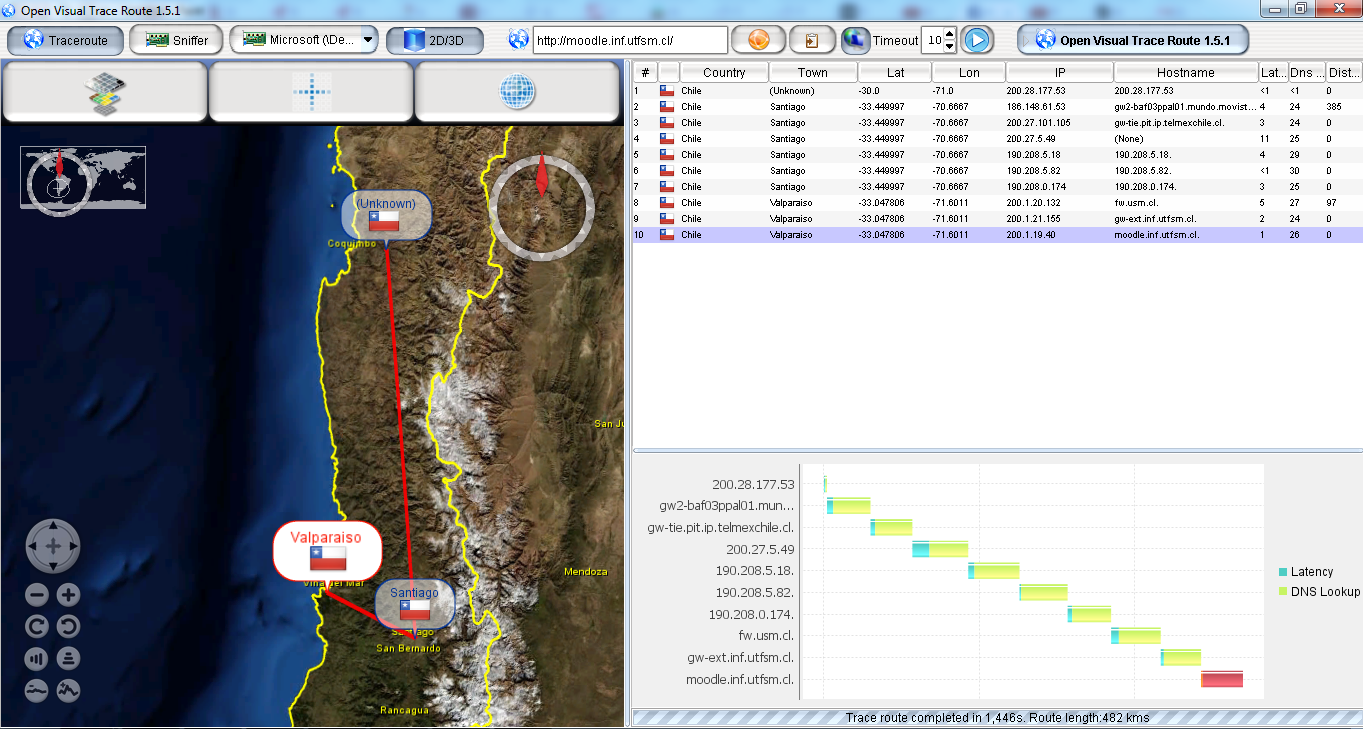
\includegraphics[scale=0.30]{tracerouteMoodle.png}
\caption{Trace Route de moodle.inf.utfsm.cl}
\label{fig:moodle}
\end{figure}  


\item[Google.cl] \hfill \\
Se ingresó http://google.cl/ a Open Visual Trace Route, el cual mostró las rutas tomadas para llevar al server final

\begin{figure}[h!]
\centering
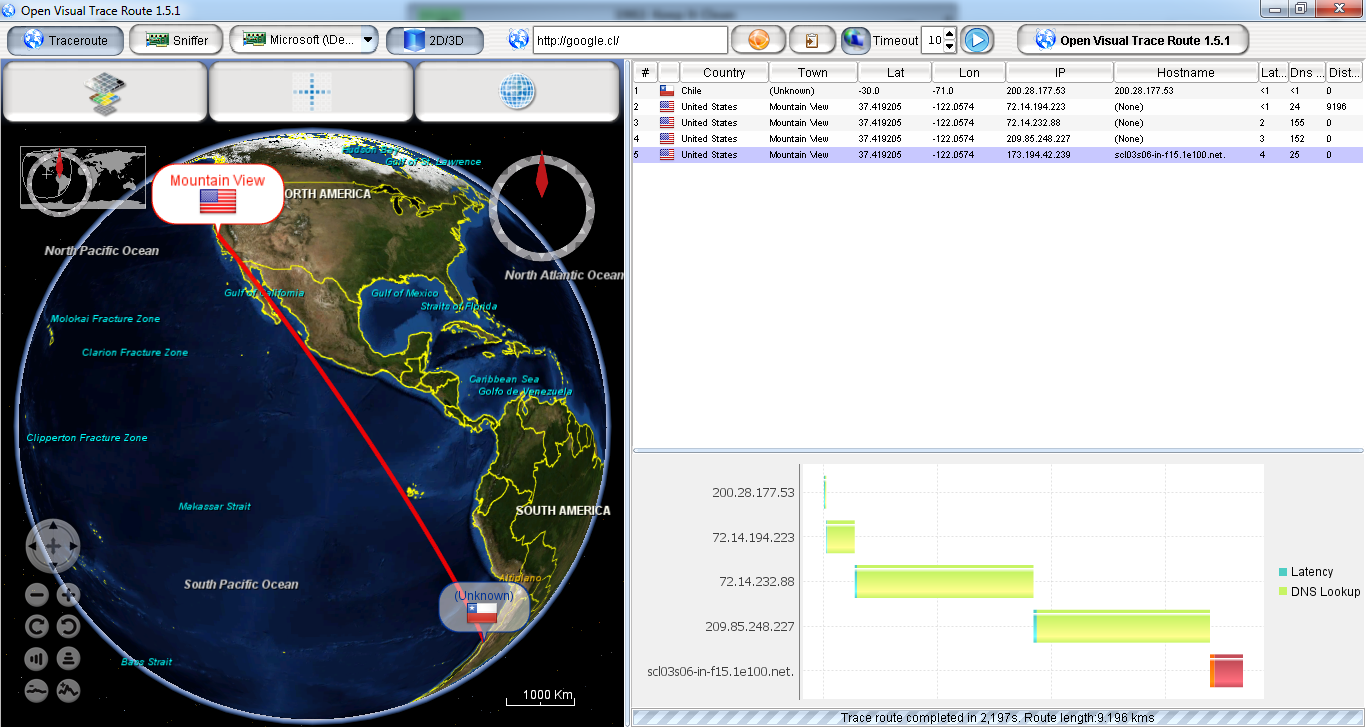
\includegraphics[scale=0.30]{tracerouteGoogleCL.png}
\caption{Trace Route de google.cl}
\label{fig:google}
\end{figure}    
  
  
\item[Cime] \hfill \\
Se ingresó http://cime.cl/ a Open Visual Trace Route, el cual mostró las rutas tomadas para llevar al server final

\begin{figure}[h!]
\centering
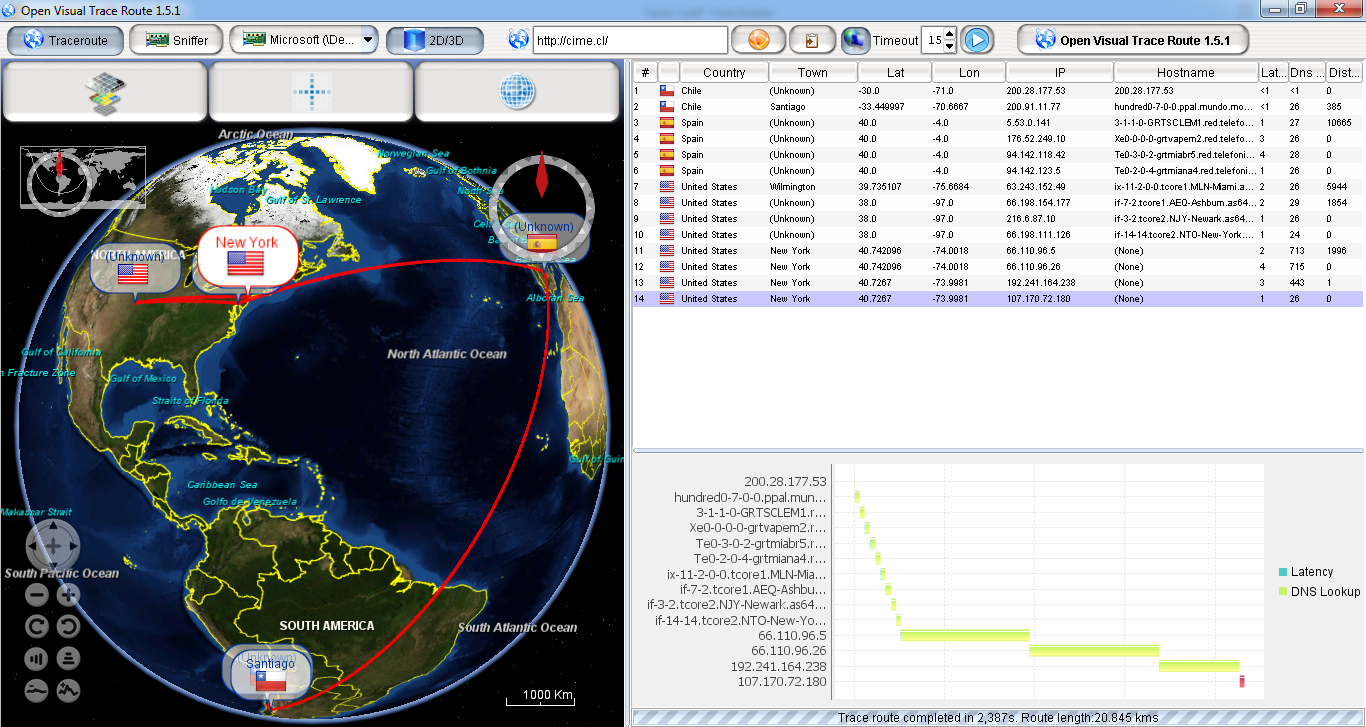
\includegraphics[scale=0.30]{tracerouteCime.png}
\caption{Trace Route de cime.cl}
\label{fig:cime}
\end{figure}    

  
\item[Wikipedia] \hfill \\
Se ingresó http://wikipedia.com/ a Open Visual Trace Route, el cual mostró las rutas tomadas para llevar al server final

\begin{figure}[h!]
\centering
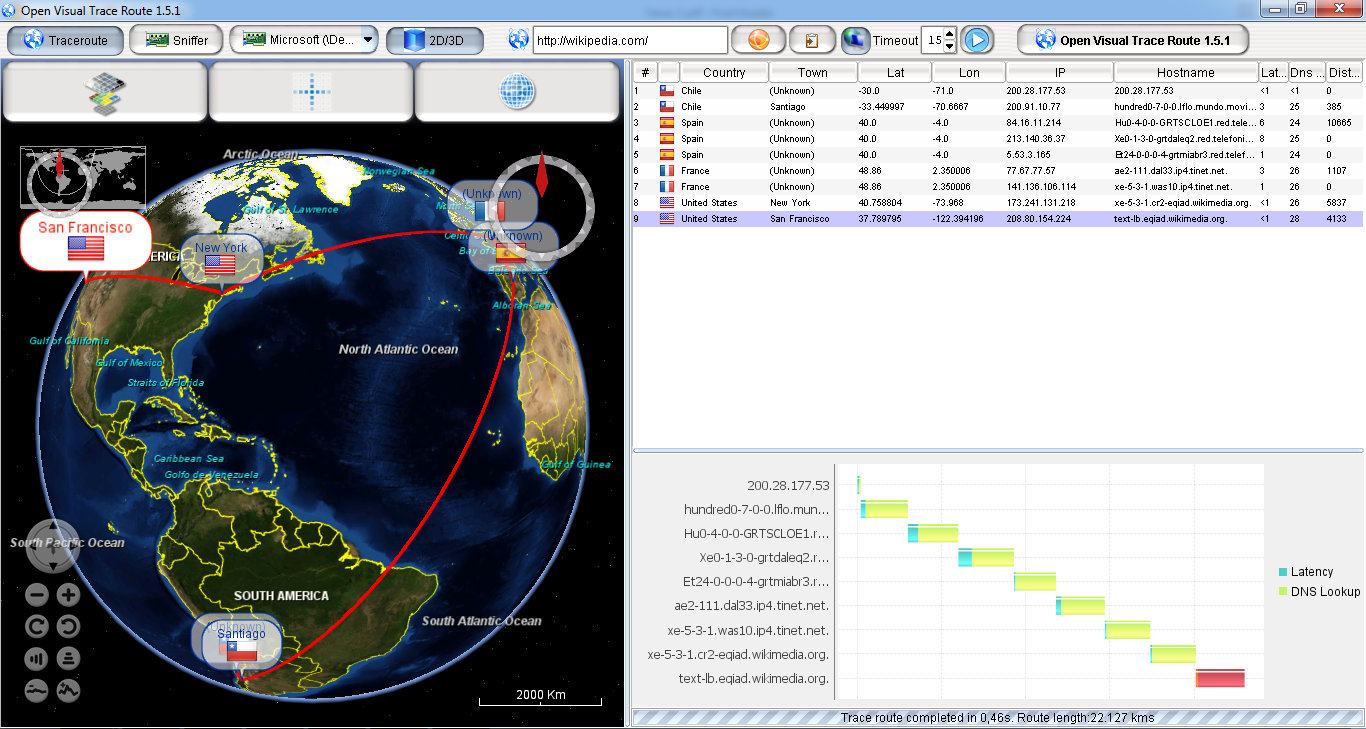
\includegraphics[scale=0.30]{tracerouteWikipedia.png}
\caption{Trace Route de wikipedia.com}
\label{fig:wikipedia}
\end{figure}    
  
  
\item[Embajada de Australia - Chile] \hfill \\
Se ingresó http://www.chile.embassy.gov.au/ a Open Visual Trace Route, el cual mostró las rutas tomadas por los paquetes. En este caso, nunca llegaron los paquetes a un destino final. Esta particular situacion se da cuando hay un firewall bloqueando ciertos tipos de mensajes ICMP. Esto se hace principalmente para protegerse de ataques DoS.

\begin{figure}[h!]
\centering
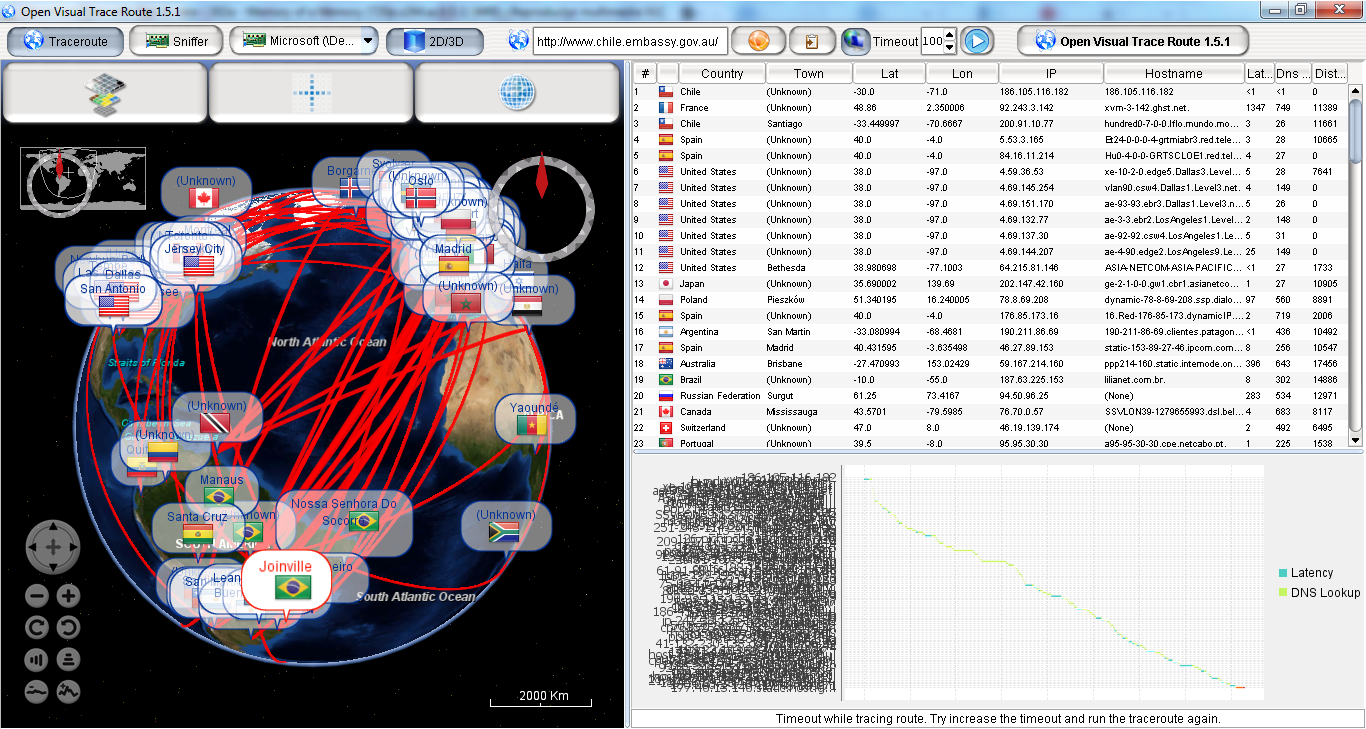
\includegraphics[scale=0.30]{traceroute_australia.png}
\caption{Trace Route de chile.embassy.gov.au}
\label{fig:embajadaChilena}
\end{figure}  

\end{description}

\clearpage

\subsection{Parte 2: "Tabla de costos routers"}
Para obtener las tablas de costos de todos los routers mediante el algoritmo vector distancia debemos realizar una serie de iteraciones, las cuales seran explicadas paso a paso

\subsubsection*{Primera Iteración: Inicialización inicial tablas de costos}
Primero se debe inicializar la tabla de costos de cada router de la siguiente manera: Sea x el router al cual se le esta calculando la tabla de costes, en la fila de x se registran los costes para ir de x a todos los demas routers (columnas), si el router es vecino, se registra el costo, si no, se marca como $\infty$ al igual que todas las demas filas que no correspondan al router x. A continuación se muestra la primera iteracion para cada tabla de costos de la red ilustrada anteriormente, quedando las siguientes tablas:\\
\\
Para la tabla del router A:\\
\begin{tabular}{ | c | c | c | c | c | c | c | c | c | c |}
\hline                 
ROUTER A    & A      & B      & C      & D      & E      & F      & G      & H      & I      \\
\hline
        A   & 0      & 1      &$\infty$&$\infty$&$\infty$&$\infty$& 4      &$\infty$& 10     \\
\hline
        B   &$\infty$&$\infty$&$\infty$&$\infty$&$\infty$&$\infty$&$\infty$&$\infty$&$\infty$\\
\hline
        C   &$\infty$&$\infty$&$\infty$&$\infty$&$\infty$&$\infty$&$\infty$&$\infty$&$\infty$\\
\hline
        D   &$\infty$&$\infty$&$\infty$&$\infty$&$\infty$&$\infty$&$\infty$&$\infty$&$\infty$\\
\hline
        E   &$\infty$&$\infty$&$\infty$&$\infty$&$\infty$&$\infty$&$\infty$&$\infty$&$\infty$\\
\hline
        F   &$\infty$&$\infty$&$\infty$&$\infty$&$\infty$&$\infty$&$\infty$&$\infty$&$\infty$\\
\hline
        G   &$\infty$&$\infty$&$\infty$&$\infty$&$\infty$&$\infty$&$\infty$&$\infty$&$\infty$\\
\hline
        H   &$\infty$&$\infty$&$\infty$&$\infty$&$\infty$&$\infty$&$\infty$&$\infty$&$\infty$\\
\hline 
        I   &$\infty$&$\infty$&$\infty$&$\infty$&$\infty$&$\infty$&$\infty$&$\infty$&$\infty$\\
\hline
\end{tabular}
\\\\
Para la tabla del router B:\\
\begin{tabular}{ | c | c | c | c | c | c | c | c | c | c |}
\hline                 
ROUTER B    & A      & B      & C      & D      & E      & F      & G      & H      & I      \\
\hline
        A   &$\infty$&$\infty$&$\infty$&$\infty$&$\infty$&$\infty$&$\infty$&$\infty$&$\infty$\\
\hline
        B   & 1      & 0      & 9      &$\infty$& 8      &$\infty$&$\infty$&$\infty$&$\infty$\\
\hline
        C   &$\infty$&$\infty$&$\infty$&$\infty$&$\infty$&$\infty$&$\infty$&$\infty$&$\infty$\\
\hline
        D   &$\infty$&$\infty$&$\infty$&$\infty$&$\infty$&$\infty$&$\infty$&$\infty$&$\infty$\\
\hline
        E   &$\infty$&$\infty$&$\infty$&$\infty$&$\infty$&$\infty$&$\infty$&$\infty$&$\infty$\\
\hline
        F   &$\infty$&$\infty$&$\infty$&$\infty$&$\infty$&$\infty$&$\infty$&$\infty$&$\infty$\\
\hline
        G   &$\infty$&$\infty$&$\infty$&$\infty$&$\infty$&$\infty$&$\infty$&$\infty$&$\infty$\\
\hline
        H   &$\infty$&$\infty$&$\infty$&$\infty$&$\infty$&$\infty$&$\infty$&$\infty$&$\infty$\\
\hline 
        I   &$\infty$&$\infty$&$\infty$&$\infty$&$\infty$&$\infty$&$\infty$&$\infty$&$\infty$\\
\hline
\end{tabular}
\\\\
Para la tabla del router C:\\
\begin{tabular}{ | c | c | c | c | c | c | c | c | c | c | c | c |}
\hline                 
ROUTER C    & A      & B      & C      & D      & E      & F      & G      & H      & I      \\
\hline
        A   &$\infty$&$\infty$&$\infty$&$\infty$&$\infty$&$\infty$&$\infty$&$\infty$&$\infty$\\
\hline
        B   &$\infty$&$\infty$&$\infty$&$\infty$&$\infty$&$\infty$&$\infty$&$\infty$&$\infty$\\
\hline
        C   &$\infty$& 9      & 0      & 2      &$\infty$&$\infty$&$\infty$&$\infty$&$\infty$\\
\hline
        D   &$\infty$&$\infty$&$\infty$&$\infty$&$\infty$&$\infty$&$\infty$&$\infty$&$\infty$\\
\hline
        E   &$\infty$&$\infty$&$\infty$&$\infty$&$\infty$&$\infty$&$\infty$&$\infty$&$\infty$\\
\hline
        F   &$\infty$&$\infty$&$\infty$&$\infty$&$\infty$&$\infty$&$\infty$&$\infty$&$\infty$\\
\hline
        G   &$\infty$&$\infty$&$\infty$&$\infty$&$\infty$&$\infty$&$\infty$&$\infty$&$\infty$\\
\hline
        H   &$\infty$&$\infty$&$\infty$&$\infty$&$\infty$&$\infty$&$\infty$&$\infty$&$\infty$\\
\hline 
        I   &$\infty$&$\infty$&$\infty$&$\infty$&$\infty$&$\infty$&$\infty$&$\infty$&$\infty$\\
\hline
\end{tabular}
\\\\
Para la tabla del router D:\\
\begin{tabular}{ | c | c | c | c | c | c | c | c | c | c |}
\hline                 
ROUTER D    & A      & B      & C      & D      & E      & F      & G      & H      & I      \\
\hline
        A   &$\infty$&$\infty$&$\infty$&$\infty$&$\infty$&$\infty$&$\infty$&$\infty$&$\infty$\\
\hline
        B   &$\infty$&$\infty$&$\infty$&$\infty$&$\infty$&$\infty$&$\infty$&$\infty$&$\infty$\\
\hline
        C   &$\infty$&$\infty$&$\infty$&$\infty$&$\infty$&$\infty$&$\infty$&$\infty$&$\infty$\\
\hline
        D   &$\infty$&$\infty$& 2      & 0      & 9      & 4      &$\infty$&$\infty$& 2      \\
\hline
        E   &$\infty$&$\infty$&$\infty$&$\infty$&$\infty$&$\infty$&$\infty$&$\infty$&$\infty$\\
\hline
        F   &$\infty$&$\infty$&$\infty$&$\infty$&$\infty$&$\infty$&$\infty$&$\infty$&$\infty$\\
\hline
        G   &$\infty$&$\infty$&$\infty$&$\infty$&$\infty$&$\infty$&$\infty$&$\infty$&$\infty$\\
\hline
        H   &$\infty$&$\infty$&$\infty$&$\infty$&$\infty$&$\infty$&$\infty$&$\infty$&$\infty$\\
\hline 
        I   &$\infty$&$\infty$&$\infty$&$\infty$&$\infty$&$\infty$&$\infty$&$\infty$&$\infty$\\
\hline
\end{tabular}
\\\\
Para la tabla del router E:\\
\begin{tabular}{ | c | c | c | c | c | c | c | c | c | c |}
\hline                 
ROUTER E    & A      & B      & C      & D      & E      & F      & G      & H      & I      \\
\hline
        A   &$\infty$&$\infty$&$\infty$&$\infty$&$\infty$&$\infty$&$\infty$&$\infty$&$\infty$\\
\hline
        B   &$\infty$&$\infty$&$\infty$&$\infty$&$\infty$&$\infty$&$\infty$&$\infty$&$\infty$\\
\hline
        C   &$\infty$&$\infty$&$\infty$&$\infty$&$\infty$&$\infty$&$\infty$&$\infty$&$\infty$\\
\hline
        D   &$\infty$&$\infty$&$\infty$&$\infty$&$\infty$&$\infty$&$\infty$&$\infty$&$\infty$\\
\hline
        E   &$\infty$& 8      &$\infty$& 9      & 0      & 2      &$\infty$&$\infty$& 1      \\
\hline
        F   &$\infty$&$\infty$&$\infty$&$\infty$&$\infty$&$\infty$&$\infty$&$\infty$&$\infty$\\
\hline
        G   &$\infty$&$\infty$&$\infty$&$\infty$&$\infty$&$\infty$&$\infty$&$\infty$&$\infty$\\
\hline
        H   &$\infty$&$\infty$&$\infty$&$\infty$&$\infty$&$\infty$&$\infty$&$\infty$&$\infty$\\
\hline 
        I   &$\infty$&$\infty$&$\infty$&$\infty$&$\infty$&$\infty$&$\infty$&$\infty$&$\infty$\\
\hline
\end{tabular}
\\\\
Para la tabla del router F:\\
\begin{tabular}{ | c | c | c | c | c | c | c | c | c | c |}
\hline                 
ROUTER F    & A      & B      & C      & D      & E      & F      & G      & H      & I      \\
\hline
        A   &$\infty$&$\infty$&$\infty$&$\infty$&$\infty$&$\infty$&$\infty$&$\infty$&$\infty$\\
\hline
        B   &$\infty$&$\infty$&$\infty$&$\infty$&$\infty$&$\infty$&$\infty$&$\infty$&$\infty$\\
\hline
        C   &$\infty$&$\infty$&$\infty$&$\infty$&$\infty$&$\infty$&$\infty$&$\infty$&$\infty$\\
\hline
        D   &$\infty$&$\infty$&$\infty$&$\infty$&$\infty$&$\infty$&$\infty$&$\infty$&$\infty$\\
\hline
        E   &$\infty$&$\infty$&$\infty$&$\infty$&$\infty$&$\infty$&$\infty$&$\infty$&$\infty$\\
\hline
        F   &$\infty$&$\infty$&$\infty$& 4      & 2      & 0      &$\infty$& 6      &$\infty$\\
\hline
        G   &$\infty$&$\infty$&$\infty$&$\infty$&$\infty$&$\infty$&$\infty$&$\infty$&$\infty$\\
\hline
        H   &$\infty$&$\infty$&$\infty$&$\infty$&$\infty$&$\infty$&$\infty$&$\infty$&$\infty$\\
\hline 
        I   &$\infty$&$\infty$&$\infty$&$\infty$&$\infty$&$\infty$&$\infty$&$\infty$&$\infty$\\
\hline
\end{tabular}
\\\\
Para la tabla del router G:\\
\begin{tabular}{ | c | c | c | c | c | c | c | c | c | c |}
\hline                 
ROUTER G    & A      & B      & C      & D      & E      & F      & G      & H      & I      \\
\hline
        A   &$\infty$&$\infty$&$\infty$&$\infty$&$\infty$&$\infty$&$\infty$&$\infty$&$\infty$\\
\hline
        B   &$\infty$&$\infty$&$\infty$&$\infty$&$\infty$&$\infty$&$\infty$&$\infty$&$\infty$\\
\hline
        C   &$\infty$&$\infty$&$\infty$&$\infty$&$\infty$&$\infty$&$\infty$&$\infty$&$\infty$\\
\hline
        D   &$\infty$&$\infty$&$\infty$&$\infty$&$\infty$&$\infty$&$\infty$&$\infty$&$\infty$\\
\hline
        E   &$\infty$&$\infty$&$\infty$&$\infty$&$\infty$&$\infty$&$\infty$&$\infty$&$\infty$\\
\hline
        F   &$\infty$&$\infty$&$\infty$&$\infty$&$\infty$&$\infty$&$\infty$&$\infty$&$\infty$\\
\hline
        G   & 4      &$\infty$&$\infty$&$\infty$&$\infty$&$\infty$& 0      & 7      &$\infty$\\
\hline
        H   &$\infty$&$\infty$&$\infty$&$\infty$&$\infty$&$\infty$&$\infty$&$\infty$&$\infty$\\
\hline 
        I   &$\infty$&$\infty$&$\infty$&$\infty$&$\infty$&$\infty$&$\infty$&$\infty$&$\infty$\\
\hline
\end{tabular}
\\\\
Para la tabla del router H:\\
\begin{tabular}{ | c | c | c | c | c | c | c | c | c | c | c | c |}
\hline                 
ROUTER H    & A      & B      & C      & D      & E      & F      & G      & H      & I      \\
\hline
        A   &$\infty$&$\infty$&$\infty$&$\infty$&$\infty$&$\infty$&$\infty$&$\infty$&$\infty$\\
\hline
        B   &$\infty$&$\infty$&$\infty$&$\infty$&$\infty$&$\infty$&$\infty$&$\infty$&$\infty$\\
\hline
        C   &$\infty$&$\infty$&$\infty$&$\infty$&$\infty$&$\infty$&$\infty$&$\infty$&$\infty$\\
\hline
        D   &$\infty$&$\infty$&$\infty$&$\infty$&$\infty$&$\infty$&$\infty$&$\infty$&$\infty$\\
\hline
        E   &$\infty$&$\infty$&$\infty$&$\infty$&$\infty$&$\infty$&$\infty$&$\infty$&$\infty$\\
\hline
        F   &$\infty$&$\infty$&$\infty$&$\infty$&$\infty$&$\infty$&$\infty$&$\infty$&$\infty$\\
\hline
        G   &$\infty$&$\infty$&$\infty$&$\infty$&$\infty$&$\infty$&$\infty$&$\infty$&$\infty$\\
\hline
        H   &$\infty$&$\infty$&$\infty$&$\infty$&$\infty$& 6      & 7      & 0      & 3      \\
\hline 
        I   &$\infty$&$\infty$&$\infty$&$\infty$&$\infty$&$\infty$&$\infty$&$\infty$&$\infty$\\
\hline
\end{tabular}
\\\\
Para la tabla del router I:\\
\begin{tabular}{ | c | c | c | c | c | c | c | c | c | c |}
\hline                 
ROUTER I    & A      & B      & C      & D      & E      & F      & G      & H      & I      \\
\hline
        A   &$\infty$&$\infty$&$\infty$&$\infty$&$\infty$&$\infty$&$\infty$&$\infty$&$\infty$\\
\hline
        B   &$\infty$&$\infty$&$\infty$&$\infty$&$\infty$&$\infty$&$\infty$&$\infty$&$\infty$\\
\hline
        C   &$\infty$&$\infty$&$\infty$&$\infty$&$\infty$&$\infty$&$\infty$&$\infty$&$\infty$\\
\hline
        D   &$\infty$&$\infty$&$\infty$&$\infty$&$\infty$&$\infty$&$\infty$&$\infty$&$\infty$\\
\hline
        E   &$\infty$&$\infty$&$\infty$&$\infty$&$\infty$&$\infty$&$\infty$&$\infty$&$\infty$\\
\hline
        F   &$\infty$&$\infty$&$\infty$&$\infty$&$\infty$&$\infty$&$\infty$&$\infty$&$\infty$\\
\hline
        G   &$\infty$&$\infty$&$\infty$&$\infty$&$\infty$&$\infty$&$\infty$&$\infty$&$\infty$\\
\hline
        H   &$\infty$&$\infty$&$\infty$&$\infty$&$\infty$&$\infty$&$\infty$&$\infty$&$\infty$\\
\hline 
        I   & 10     &$\infty$&$\infty$& 2      & 1      &$\infty$&$\infty$& 3      & 0      \\
\hline
\end{tabular}

\subsubsection*{Segunda Iteración: Actualizacion de tablas de costos con tablas de vecinos}
En esta parte cada router le informa a sus vecinos su tabla de costos, actualizandose los costos, como es la primera iteracion despues de la iteracion inicial, no hay cambios con los costos informados pues todos son mejores que los cosotos de $\infty$ que se generaron en la primera iteración. Las tablas de costos quedan entonces de la siguiente forma:\\
\\
Para la tabla del router A:\\
\begin{tabular}{ | c | c | c | c | c | c | c | c | c | c |}
\hline                 
ROUTER A    & A      & B      & C      & D      & E      & F      & G      & H      & I      \\
\hline
        A   & 0      & 1      &10      &$\infty$& 9      &$\infty$& 4      &$\infty$& 10     \\
\hline
        B   & 1      & 0      & 9      &$\infty$& 8      &$\infty$& 5      &$\infty$& 11     \\
\hline
        C   & 10     & 9      & 18     &$\infty$& 17     &$\infty$&$\infty$&$\infty$&$\infty$\\
\hline
        D   &$\infty$&$\infty$&$\infty$&$\infty$&$\infty$&$\infty$&$\infty$&$\infty$&$\infty$\\
\hline
        E   & 9      & 8      & 17     &$\infty$& 16     &$\infty$&$\infty$&$\infty$&$\infty$\\
\hline
        F   &$\infty$&$\infty$&$\infty$&$\infty$&$\infty$&$\infty$&$\infty$&$\infty$&$\infty$\\
\hline
        G   & 4      & 5      &$\infty$&$\infty$&$\infty$&$\infty$& 8      & 14     &$\infty$\\
\hline
        H   &$\infty$&$\infty$&$\infty$&$\infty$&$\infty$&$\infty$&$\infty$&$\infty$&$\infty$\\
\hline 
        I   & 10     & 11     &$\infty$&$\infty$&$\infty$&$\infty$& 14     &$\infty$& 20     \\
\hline 
\end{tabular}
\\\\
Para la tabla del router B:\\
\begin{tabular}{ | c | c | c | c | c | c | c | c | c | c |}
\hline                 
ROUTER B    & A      & B      & C      & D      & E      & F      & G      & H      & I      \\
\hline
        A   & 0      & 1      &$\infty$&$\infty$&$\infty$&$\infty$& 4      &$\infty$& 10     \\
\hline
        B   & 1      & 0      & 9      &$\infty$& 8      &$\infty$&$\infty$&$\infty$&$\infty$\\
\hline
        C   &$\infty$& 9      & 0      & 2      &$\infty$&$\infty$&$\infty$&$\infty$&$\infty$\\
\hline
        D   &$\infty$&$\infty$&$\infty$&$\infty$&$\infty$&$\infty$&$\infty$&$\infty$&$\infty$\\
\hline
        E   &$\infty$& 8      &$\infty$& 9      & 0      & 2      &$\infty$&$\infty$& 1      \\
\hline
        F   &$\infty$&$\infty$&$\infty$&$\infty$&$\infty$&$\infty$&$\infty$&$\infty$&$\infty$\\
\hline
        G   &$\infty$&$\infty$&$\infty$&$\infty$&$\infty$&$\infty$&$\infty$&$\infty$&$\infty$\\
\hline
        H   &$\infty$&$\infty$&$\infty$&$\infty$&$\infty$&$\infty$&$\infty$&$\infty$&$\infty$\\
\hline 
        I   &$\infty$&$\infty$&$\infty$&$\infty$&$\infty$&$\infty$&$\infty$&$\infty$&$\infty$\\
\hline
\end{tabular}
\\\\
Para la tabla del router C:\\
\begin{tabular}{ | c | c | c | c | c | c | c | c | c | c |}
\hline                 
ROUTER C    & A      & B      & C      & D      & E      & F      & G      & H      & I      \\
\hline
        A   &$\infty$&$\infty$&$\infty$&$\infty$&$\infty$&$\infty$&$\infty$&$\infty$&$\infty$\\
\hline
        B   & 1      & 0      & 9      &$\infty$& 8      &$\infty$&$\infty$&$\infty$&$\infty$\\
\hline
        C   &$\infty$& 9      & 0      & 2      &$\infty$&$\infty$&$\infty$&$\infty$&$\infty$\\
\hline
        D   &$\infty$&$\infty$& 2      & 0      & 9      & 4      &$\infty$&$\infty$& 2      \\
\hline
        E   &$\infty$&$\infty$&$\infty$&$\infty$&$\infty$&$\infty$&$\infty$&$\infty$&$\infty$\\
\hline
        F   &$\infty$&$\infty$&$\infty$&$\infty$&$\infty$&$\infty$&$\infty$&$\infty$&$\infty$\\
\hline
        G   &$\infty$&$\infty$&$\infty$&$\infty$&$\infty$&$\infty$&$\infty$&$\infty$&$\infty$\\
\hline
        H   &$\infty$&$\infty$&$\infty$&$\infty$&$\infty$&$\infty$&$\infty$&$\infty$&$\infty$\\
\hline 
        I   &$\infty$&$\infty$&$\infty$&$\infty$&$\infty$&$\infty$&$\infty$&$\infty$&$\infty$\\
\hline
\end{tabular}
\\\\
Para la tabla del router D:\\
\begin{tabular}{ | c | c | c | c | c | c | c | c | c | c |}
\hline                 
ROUTER D    & A      & B      & C      & D      & E      & F      & G      & H      & I      \\
\hline
        A   &$\infty$&$\infty$&$\infty$&$\infty$&$\infty$&$\infty$&$\infty$&$\infty$&$\infty$\\
\hline
        B   &$\infty$&$\infty$&$\infty$&$\infty$&$\infty$&$\infty$&$\infty$&$\infty$&$\infty$\\
\hline
        C   &$\infty$& 9      & 0      & 2      &$\infty$&$\infty$&$\infty$&$\infty$&$\infty$\\
\hline
        D   &$\infty$&$\infty$& 2      & 0      & 9      & 4      &$\infty$&$\infty$& 2      \\
\hline
        E   &$\infty$& 8      &$\infty$& 9      & 0      & 2      &$\infty$&$\infty$& 1      \\
\hline
        F   &$\infty$&$\infty$&$\infty$& 4      & 2      & 0      &$\infty$& 6      &$\infty$\\
\hline
        G   &$\infty$&$\infty$&$\infty$&$\infty$&$\infty$&$\infty$&$\infty$&$\infty$&$\infty$\\
\hline
        H   &$\infty$&$\infty$&$\infty$&$\infty$&$\infty$&$\infty$&$\infty$&$\infty$&$\infty$\\
\hline 
        I   & 10     &$\infty$&$\infty$& 2      & 1      &$\infty$&$\infty$& 3      & 0      \\
\hline
\end{tabular}
\\\\
Para la tabla del router E:\\
\begin{tabular}{ | c | c | c | c | c | c | c | c | c | c |}
\hline                 
ROUTER E    & A      & B      & C      & D      & E      & F      & G      & H      & I      \\
\hline
        A   &$\infty$&$\infty$&$\infty$&$\infty$&$\infty$&$\infty$&$\infty$&$\infty$&$\infty$\\
\hline
        B   & 1      & 0      & 9      &$\infty$& 8      &$\infty$&$\infty$&$\infty$&$\infty$\\
\hline
        C   &$\infty$&$\infty$&$\infty$&$\infty$&$\infty$&$\infty$&$\infty$&$\infty$&$\infty$\\
\hline
        D   &$\infty$&$\infty$& 2      & 0      & 9      & 4      &$\infty$&$\infty$& 2      \\
\hline
        E   &$\infty$& 8      &$\infty$& 9      & 0      & 2      &$\infty$&$\infty$& 1      \\
\hline
        F   &$\infty$&$\infty$&$\infty$& 4      & 2      & 0      &$\infty$& 6      &$\infty$\\
\hline
        G   &$\infty$&$\infty$&$\infty$&$\infty$&$\infty$&$\infty$&$\infty$&$\infty$&$\infty$\\
\hline
        H   &$\infty$&$\infty$&$\infty$&$\infty$&$\infty$&$\infty$&$\infty$&$\infty$&$\infty$\\
\hline 
        I   & 10     &$\infty$&$\infty$& 2      & 1      &$\infty$&$\infty$& 3      & 0      \\
\hline
\end{tabular}
\\\\
Para la tabla del router F:\\
\begin{tabular}{ | c | c | c | c | c | c | c | c | c | c |}
\hline                 
ROUTER F    & A      & B      & C      & D      & E      & F      & G      & H      & I      \\
\hline
        A   &$\infty$&$\infty$&$\infty$&$\infty$&$\infty$&$\infty$&$\infty$&$\infty$&$\infty$\\
\hline
        B   &$\infty$&$\infty$&$\infty$&$\infty$&$\infty$&$\infty$&$\infty$&$\infty$&$\infty$\\
\hline
        C   &$\infty$&$\infty$&$\infty$&$\infty$&$\infty$&$\infty$&$\infty$&$\infty$&$\infty$\\
\hline
        D   &$\infty$&$\infty$& 2      & 0      & 9      & 4      &$\infty$&$\infty$& 2      \\
\hline
        E   &$\infty$& 8      &$\infty$& 9      & 0      & 2      &$\infty$&$\infty$& 1      \\
\hline
        F   &$\infty$&$\infty$&$\infty$& 4      & 2      & 0      &$\infty$& 6      &$\infty$\\
\hline
        G   &$\infty$&$\infty$&$\infty$&$\infty$&$\infty$&$\infty$&$\infty$&$\infty$&$\infty$\\
\hline
        H   &$\infty$&$\infty$&$\infty$&$\infty$&$\infty$& 6      & 7      & 0      & 3      \\
\hline 
        I   &$\infty$&$\infty$&$\infty$&$\infty$&$\infty$&$\infty$&$\infty$&$\infty$&$\infty$\\
\hline
\end{tabular}
\\\\
Para la tabla del router G:\\
\begin{tabular}{ | c | c | c | c | c | c | c | c | c | c |}
\hline                 
ROUTER G    & A      & B      & C      & D      & E      & F      & G      & H      & I      \\
\hline
        A   & 0      & 1      &$\infty$&$\infty$&$\infty$&$\infty$& 4      &$\infty$& 10     \\
\hline
        B   &$\infty$&$\infty$&$\infty$&$\infty$&$\infty$&$\infty$&$\infty$&$\infty$&$\infty$\\
\hline
        C   &$\infty$&$\infty$&$\infty$&$\infty$&$\infty$&$\infty$&$\infty$&$\infty$&$\infty$\\
\hline
        D   &$\infty$&$\infty$&$\infty$&$\infty$&$\infty$&$\infty$&$\infty$&$\infty$&$\infty$\\
\hline
        E   &$\infty$&$\infty$&$\infty$&$\infty$&$\infty$&$\infty$&$\infty$&$\infty$&$\infty$\\
\hline
        F   &$\infty$&$\infty$&$\infty$&$\infty$&$\infty$&$\infty$&$\infty$&$\infty$&$\infty$\\
\hline
        G   & 4      &$\infty$&$\infty$&$\infty$&$\infty$&$\infty$& 0      & 7      &$\infty$\\
\hline
        H   &$\infty$&$\infty$&$\infty$&$\infty$&$\infty$& 6      & 7      & 0      & 3      \\
\hline 
        I   &$\infty$&$\infty$&$\infty$&$\infty$&$\infty$&$\infty$&$\infty$&$\infty$&$\infty$\\
\hline
\end{tabular}
\\\\
Para la tabla del router H:\\
\begin{tabular}{ | c | c | c | c | c | c | c | c | c | c |}
\hline                 
ROUTER H    & A      & B      & C      & D      & E      & F      & G      & H      & I      \\
\hline
        A   &$\infty$&$\infty$&$\infty$&$\infty$&$\infty$&$\infty$&$\infty$&$\infty$&$\infty$\\
\hline
        B   &$\infty$&$\infty$&$\infty$&$\infty$&$\infty$&$\infty$&$\infty$&$\infty$&$\infty$\\
\hline
        C   &$\infty$&$\infty$&$\infty$&$\infty$&$\infty$&$\infty$&$\infty$&$\infty$&$\infty$\\
\hline
        D   &$\infty$&$\infty$&$\infty$&$\infty$&$\infty$&$\infty$&$\infty$&$\infty$&$\infty$\\
\hline
        E   &$\infty$&$\infty$&$\infty$&$\infty$&$\infty$&$\infty$&$\infty$&$\infty$&$\infty$\\
\hline
        F   &$\infty$&$\infty$&$\infty$& 4      & 2      & 0      &$\infty$& 6      &$\infty$\\
\hline
        G   & 4      &$\infty$&$\infty$&$\infty$&$\infty$&$\infty$& 0      & 7      &$\infty$\\
\hline
        H   &$\infty$&$\infty$&$\infty$&$\infty$&$\infty$& 6      & 7      & 0      & 3      \\
\hline 
        I   & 10     &$\infty$&$\infty$& 2      & 1      &$\infty$&$\infty$& 3      & 0      \\
\hline
\end{tabular}
\\\\
Para la tabla del router I:\\
\begin{tabular}{ | c | c | c | c | c | c | c | c | c | c |}
\hline                 
ROUTER I    & A      & B      & C      & D      & E      & F      & G      & H      & I      \\
\hline
        A   & 0      & 1      &$\infty$&$\infty$&$\infty$&$\infty$& 4      &$\infty$& 10     \\
\hline
        B   &$\infty$&$\infty$&$\infty$&$\infty$&$\infty$&$\infty$&$\infty$&$\infty$&$\infty$\\
\hline
        C   &$\infty$&$\infty$&$\infty$&$\infty$&$\infty$&$\infty$&$\infty$&$\infty$&$\infty$\\
\hline
        D   &$\infty$&$\infty$& 2      & 0      & 9      & 4      &$\infty$&$\infty$& 2      \\
\hline
        E   &$\infty$& 8      &$\infty$& 9      & 0      & 2      &$\infty$&$\infty$& 1      \\
\hline
        F   &$\infty$&$\infty$&$\infty$&$\infty$&$\infty$&$\infty$&$\infty$&$\infty$&$\infty$\\
\hline
        G   &$\infty$&$\infty$&$\infty$&$\infty$&$\infty$&$\infty$&$\infty$&$\infty$&$\infty$\\
\hline
        H   &$\infty$&$\infty$&$\infty$&$\infty$&$\infty$& 6      & 7      & 0      & 3      \\
\hline 
        I   & 10     &$\infty$&$\infty$& 2      & 1      &$\infty$&$\infty$& 3      & 0      \\
\hline
\end{tabular}

\subsubsection*{Tercera Iteración: Actualización de tablas de costos con tablas de vecinos}
Nuevamente se informa a los vecinos que hubo cambios en su tabla de costos, y se les envia la tabla, pero esta vez, como no todos los costos son $\infty$ habran cambios en algunos vectores distancia. Las tablas al realizarse esta iteracion quedan de la siguiente forma:\\
\\


\subsection{Parte 3: "NO RECUERDO QUE VA AQUI"}

\section{Conclusión}
``I always thought something was fundamentally wrong with the universe'' \citep{adams1995hitchhiker}

\bibliographystyle{plain}
\bibliography{references}
\end{document}
